\documentclass[11pt,a4paper]{article}
\usepackage[utf8]{inputenc}
\usepackage[spanish]{babel}
\usepackage{amsmath}
\usepackage{amsfonts}
\usepackage{amssymb}
\usepackage{makeidx}
\usepackage{graphicx}
\usepackage{float}
\usepackage{lmodern}
\usepackage[left=2cm,right=2cm,top=2cm,bottom=2cm]{geometry}
\author{Christopher Soto Cabezas - C17745}
\title{Tarea 03 - Física Computacional - Resolución de Ecuaciones Diferenciales mediante Métodos de Euler, RK2 y RK4}
\begin{document}
\maketitle
\section*{Introducción}
En este caso, tenemos la implementación de dos archivos completamente distintos, los cuales se encuentra datos, uno para el lenguaje \texttt{C++} y el otro para el lenguaje \texttt{Python}. En este caso, podemos observar que implementamos los métodos computacionales para cálculo de ecuaciones diferenciales a nivel numérico de Euler, Runge-Kutta 2 y Runge-Kutta 4, estos métodos se ven implementados desde \texttt{C++} y posteriormente, mediante la librería pybind11, se enlazan con Python, para poder ejecutar los métodos compilados en \texttt{C++} y obtener los respectivos resultados desde \texttt{Python}. En el archivo de \texttt{Python}, que se le dio el nombre de \texttt{main.py}, podemos encontrar los datos que se van a ingresar para la ejecución de los métodos numéricos, así como la configuración para armar las gráficas de acuerdo a los resultados obtenidos. Al no poseer propiamente una solución analítica exacta para el sistema de ecuaciones diferenciales de Lorenz, la única manera de estudiar su dinámica tridimensional y geometría del atractor de Lorenz, es mediante el analísis numérico mediante computación, en este caso, usamos los métodos de \textbf{Euler, RK2 y RK4}.
\section*{Discusión de Resultados}

\subsection*{Sensibilidad a Condiciones Iniciales}

En esta sección, procederemos a explicar un poco del comportamiento de la sensibilidad a las condiciones iniciales para Lorenz con el método de Runge-Kutta 4. En este caso, podemos observar que el programa arrojó inicialmente una sensibilidad de $1.0 \cdot 10^{-8}$ y posteriormente, aumentó drásticamente hasta llegar a periodo 40. Al contrastar los atractores tridimensionales, se evidencia un aumento de la sensibilidad al pasar el tiempo, donde para el caso de una trayectoria ideal y perturbada, podemos observar un cambio significativo a medida que avanza el tiempo. Podemos observar un fenómeno conocido como "Efecto Mariposa", donde la separación inicial resulta ser baja, y posteriormente aumenta de forma considerablemente, de acuerdo a lo observado en los datos obtenidos en \texttt{output.txt}.  \\

En el caso de la curva semi-logarítmica, podemos identificar un régimen dinámico curioso, donde hay un comportamiento ideal lineal estricto en la escala logarítmica, sin embargo, cuando passamos al tiempo $t \approx 30$, este crecimiento se detiene, donde en ese caso, aumenta la pendiente positiva de la perturbación vinculada al máximo exponente de Lyapunov del sistema. 

\begin{figure}[H]
	\centering
	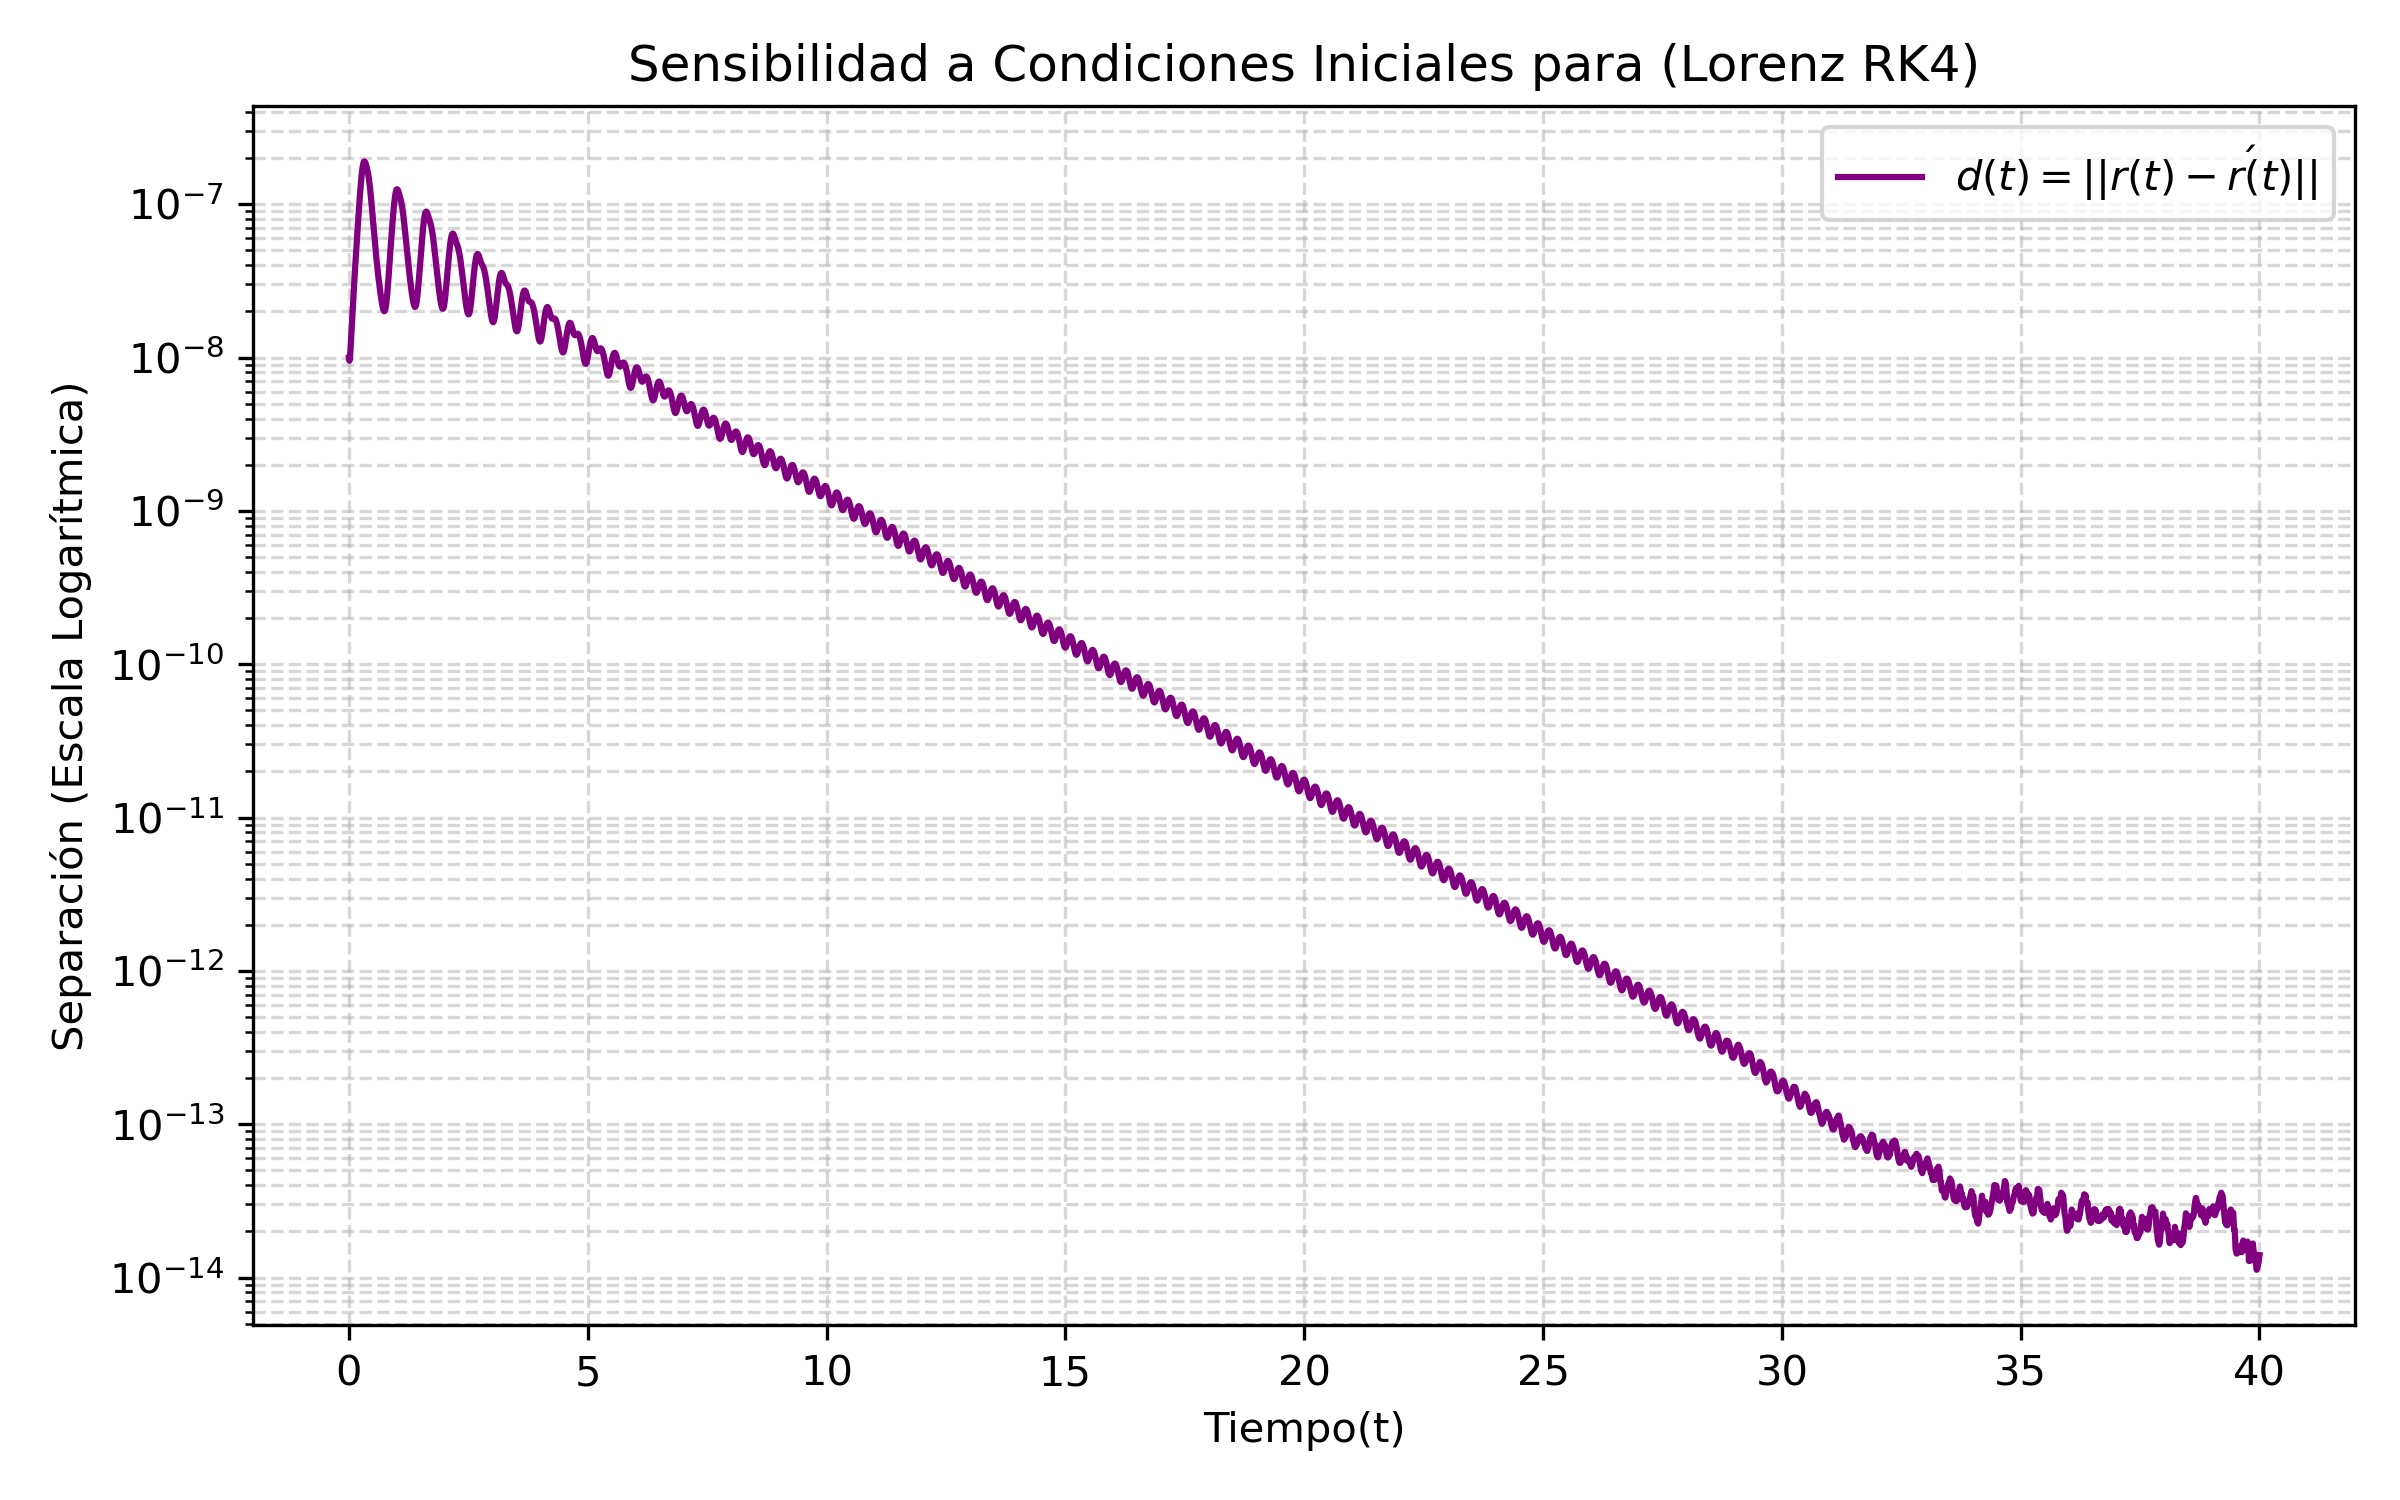
\includegraphics[scale=0.8]{sensibilidad.png}
	\caption{Evolución temporal de distancia euclídea $d(t)$ entre la trayectoria ideal y la perturbada}
	\label{fig:Sensibilidad}
\end{figure}

\subsection*{Métodos de Euler y Familia Runge-Kutta}

En el caso del comportamiento del método de Euler, podemos observar algunas limitaciones, donde en el caso del esquema de primer orden para sistemas dinámicos no acoplados, existe un error de orden $h$, donde la aproximación lineal acumula desviaciones de manera espuria a lo largo del tiempo, lo que aparece como una falsa difusión numérica que provoca trayectorias espirales que no deberían existir, por lo que el método de Euler diverge por completo de la trayectoria física real del sistema.

\begin{figure}[H]
	\centering
	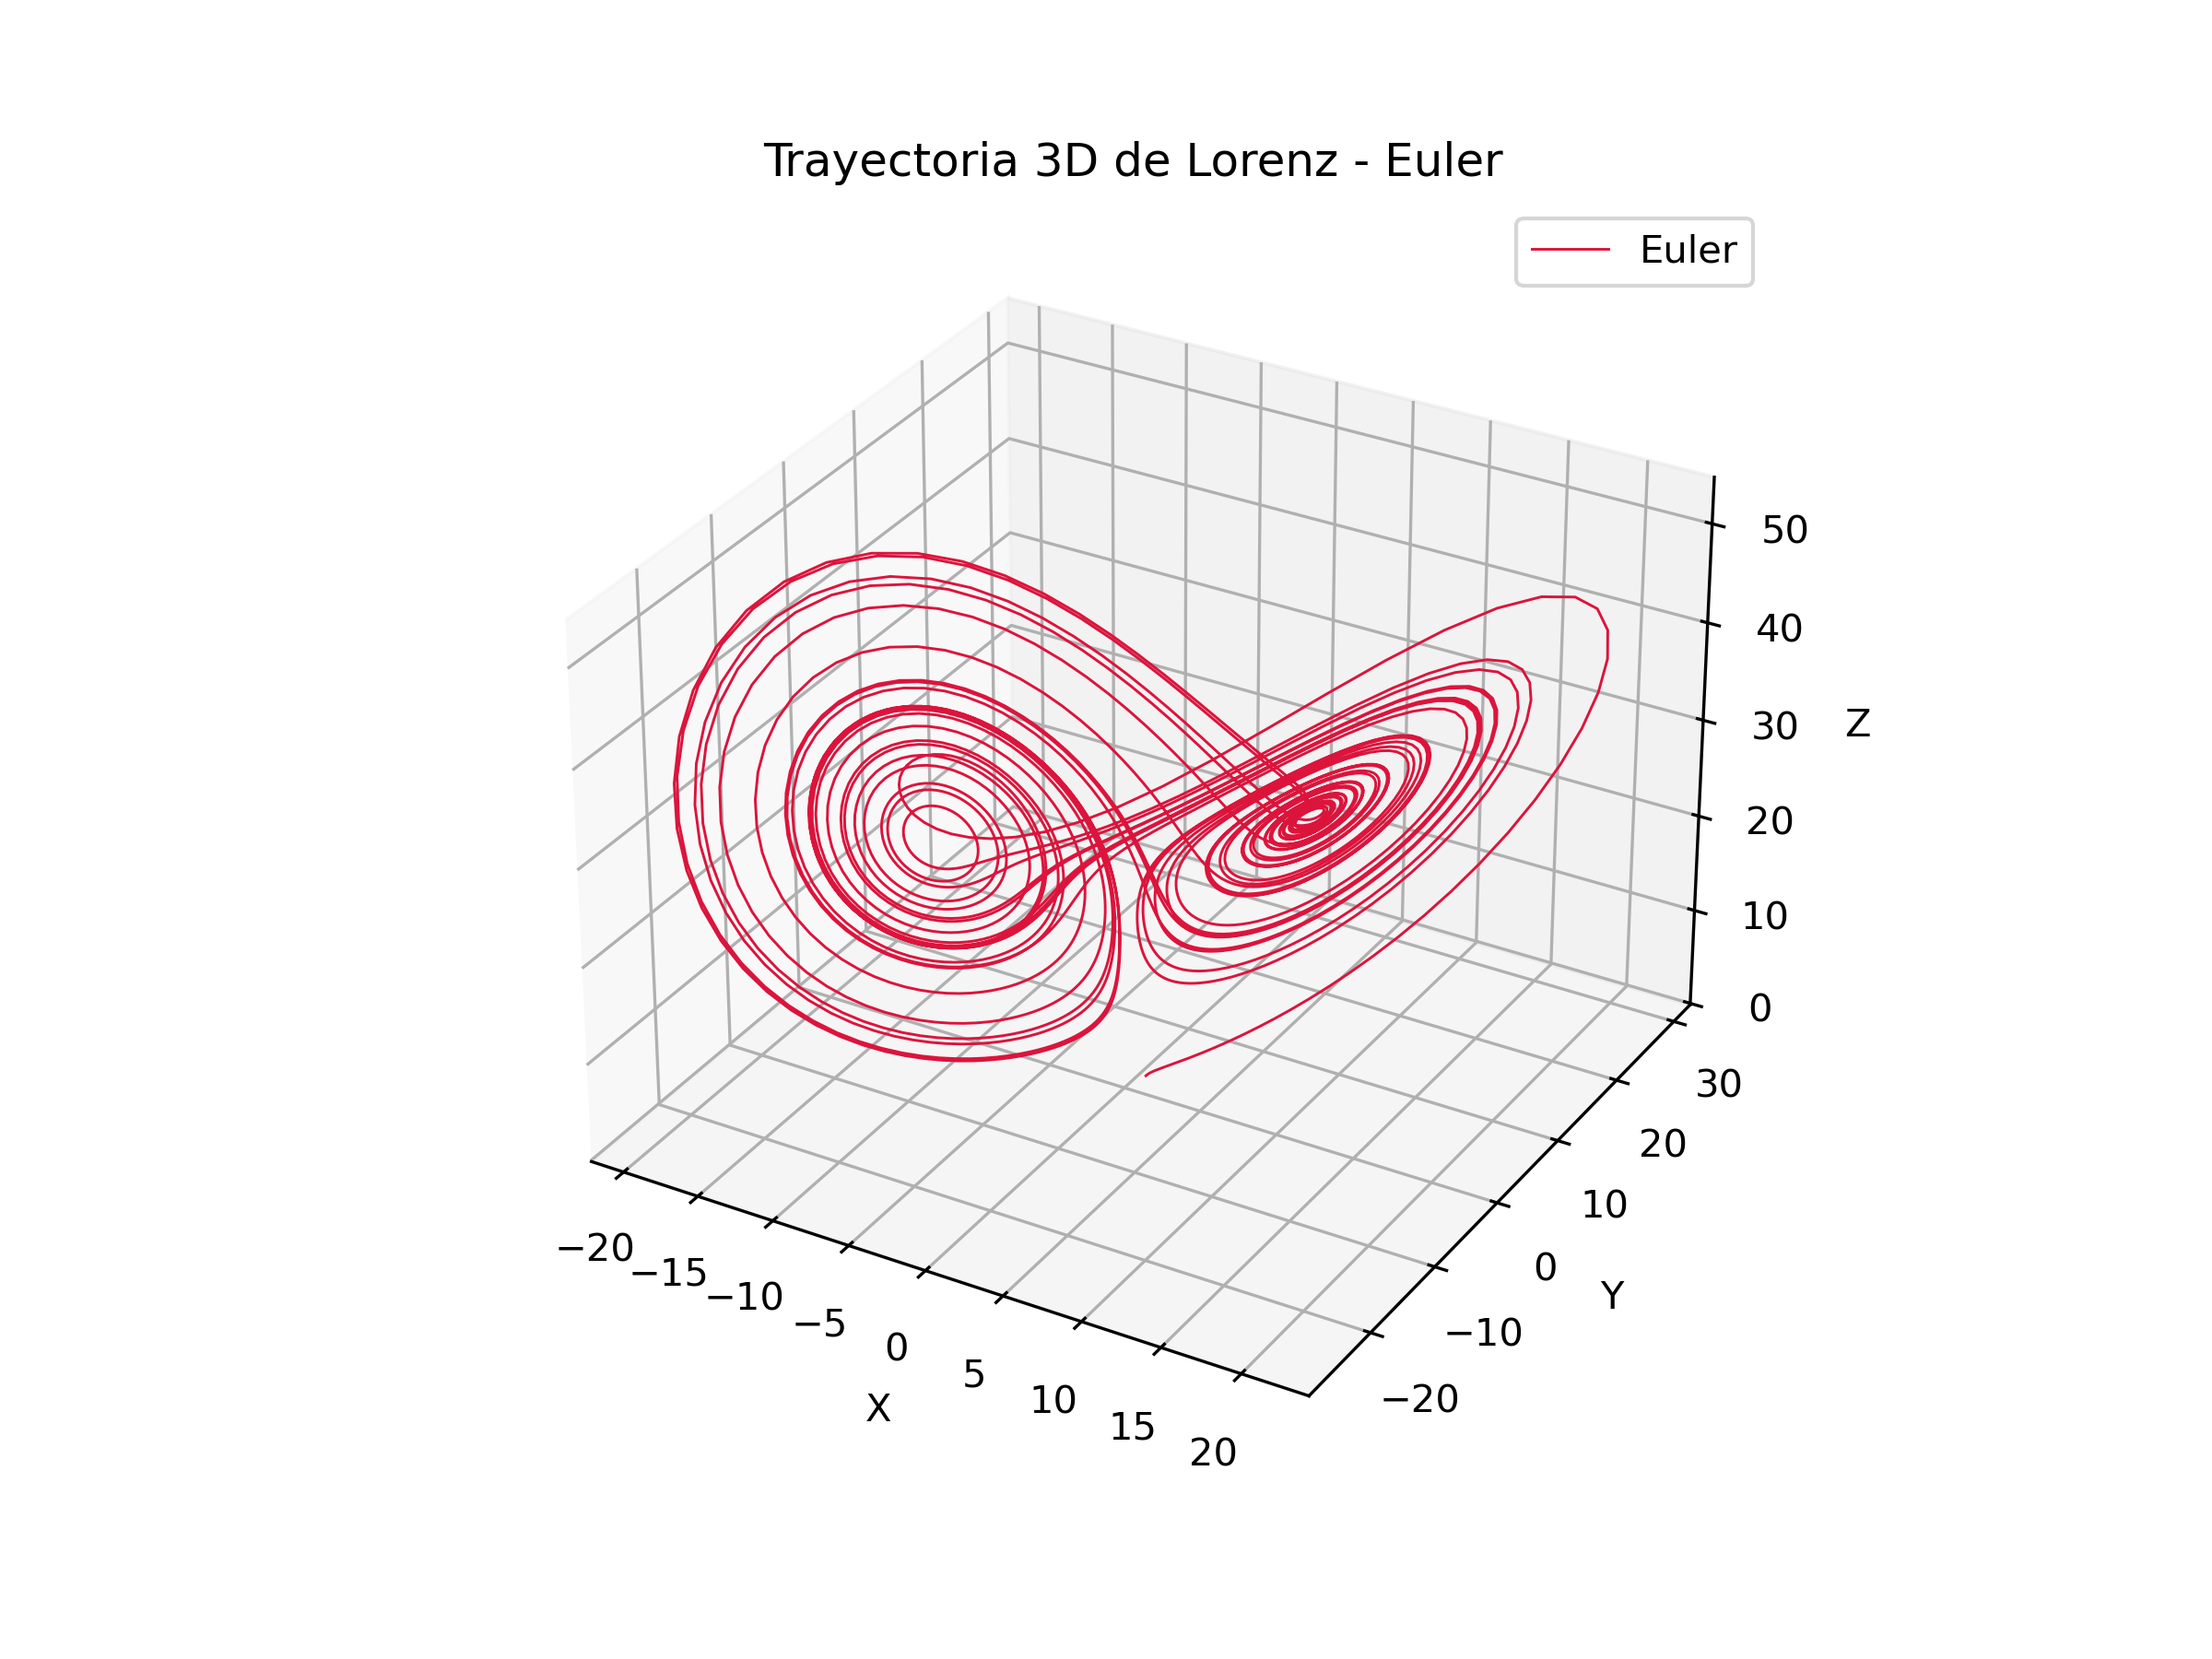
\includegraphics[scale=0.8]{trayectoria_3d_euler.png}
	\caption{Resultado de la solución de ecuaciones diferenciales (trayectoria) mediante el método de Euler}
	\label{fig:Euler}
\end{figure}

Los métodos de la familia Runge-Kutta muestran por el contrario, una enorme estabilidad geométrica notablemente superior al método de Euler, donde para el caso de RK2, podemos observar una mitigación de la divergencia matemática inmediata reduciendo el error global $\mathcal{O}(h^2)$. \\

Para el caso de RK4, es el que produce con mayor fidelidad el funcionamiento y recorrido "extraño" del atractor de Lorenz, donde al promediar las cuatro pendientes en subintervalos actoados, RK4 alcanza una precisión global de orden $\mathcal{O}(h^4)$, lo que permite retener órbitas aperiódicas alrededor de puntos fijos sin exhibir decaimiento o disipación artificial como la observada con el Método de Euler. \\

\begin{figure}[H]
	\centering
	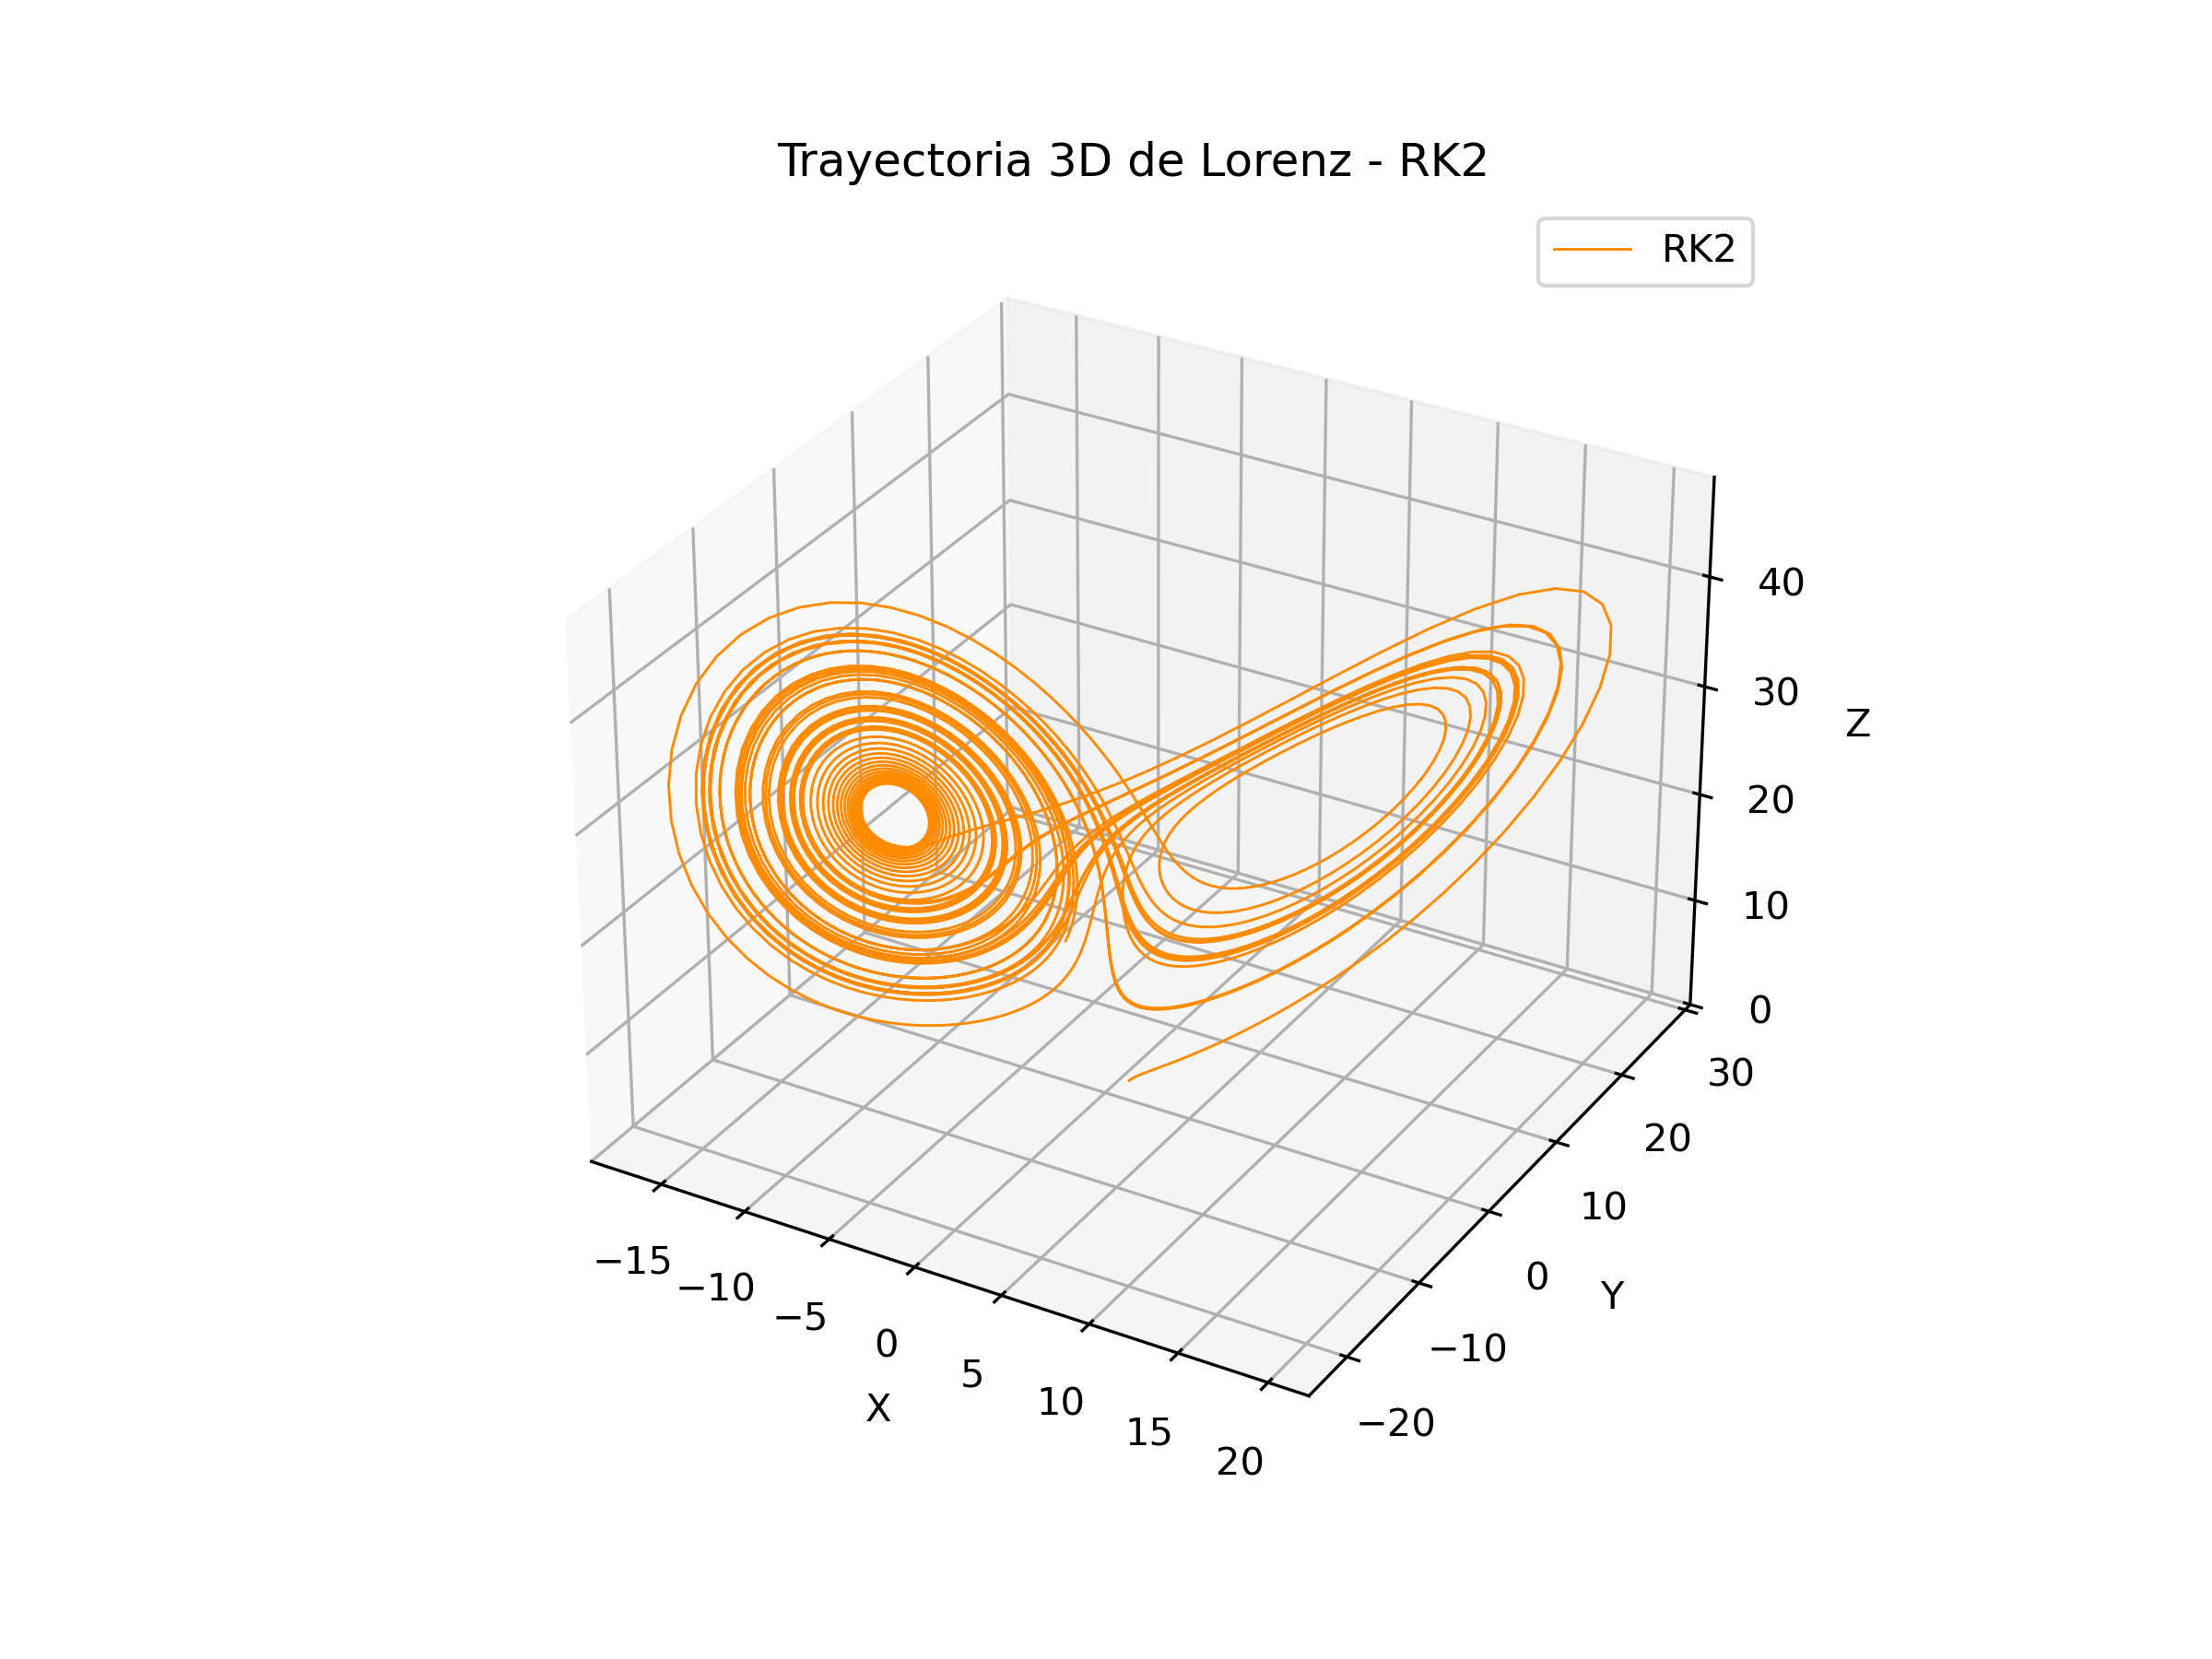
\includegraphics[scale=0.8]{trayectoria_3d_rk2.png}
	\caption{Resultado de la solución de ecuaciones diferenciales (trayectoria) mediante el método RK2}
	\label{fig:RK2}
\end{figure}



\begin{figure}[H]
	\centering
	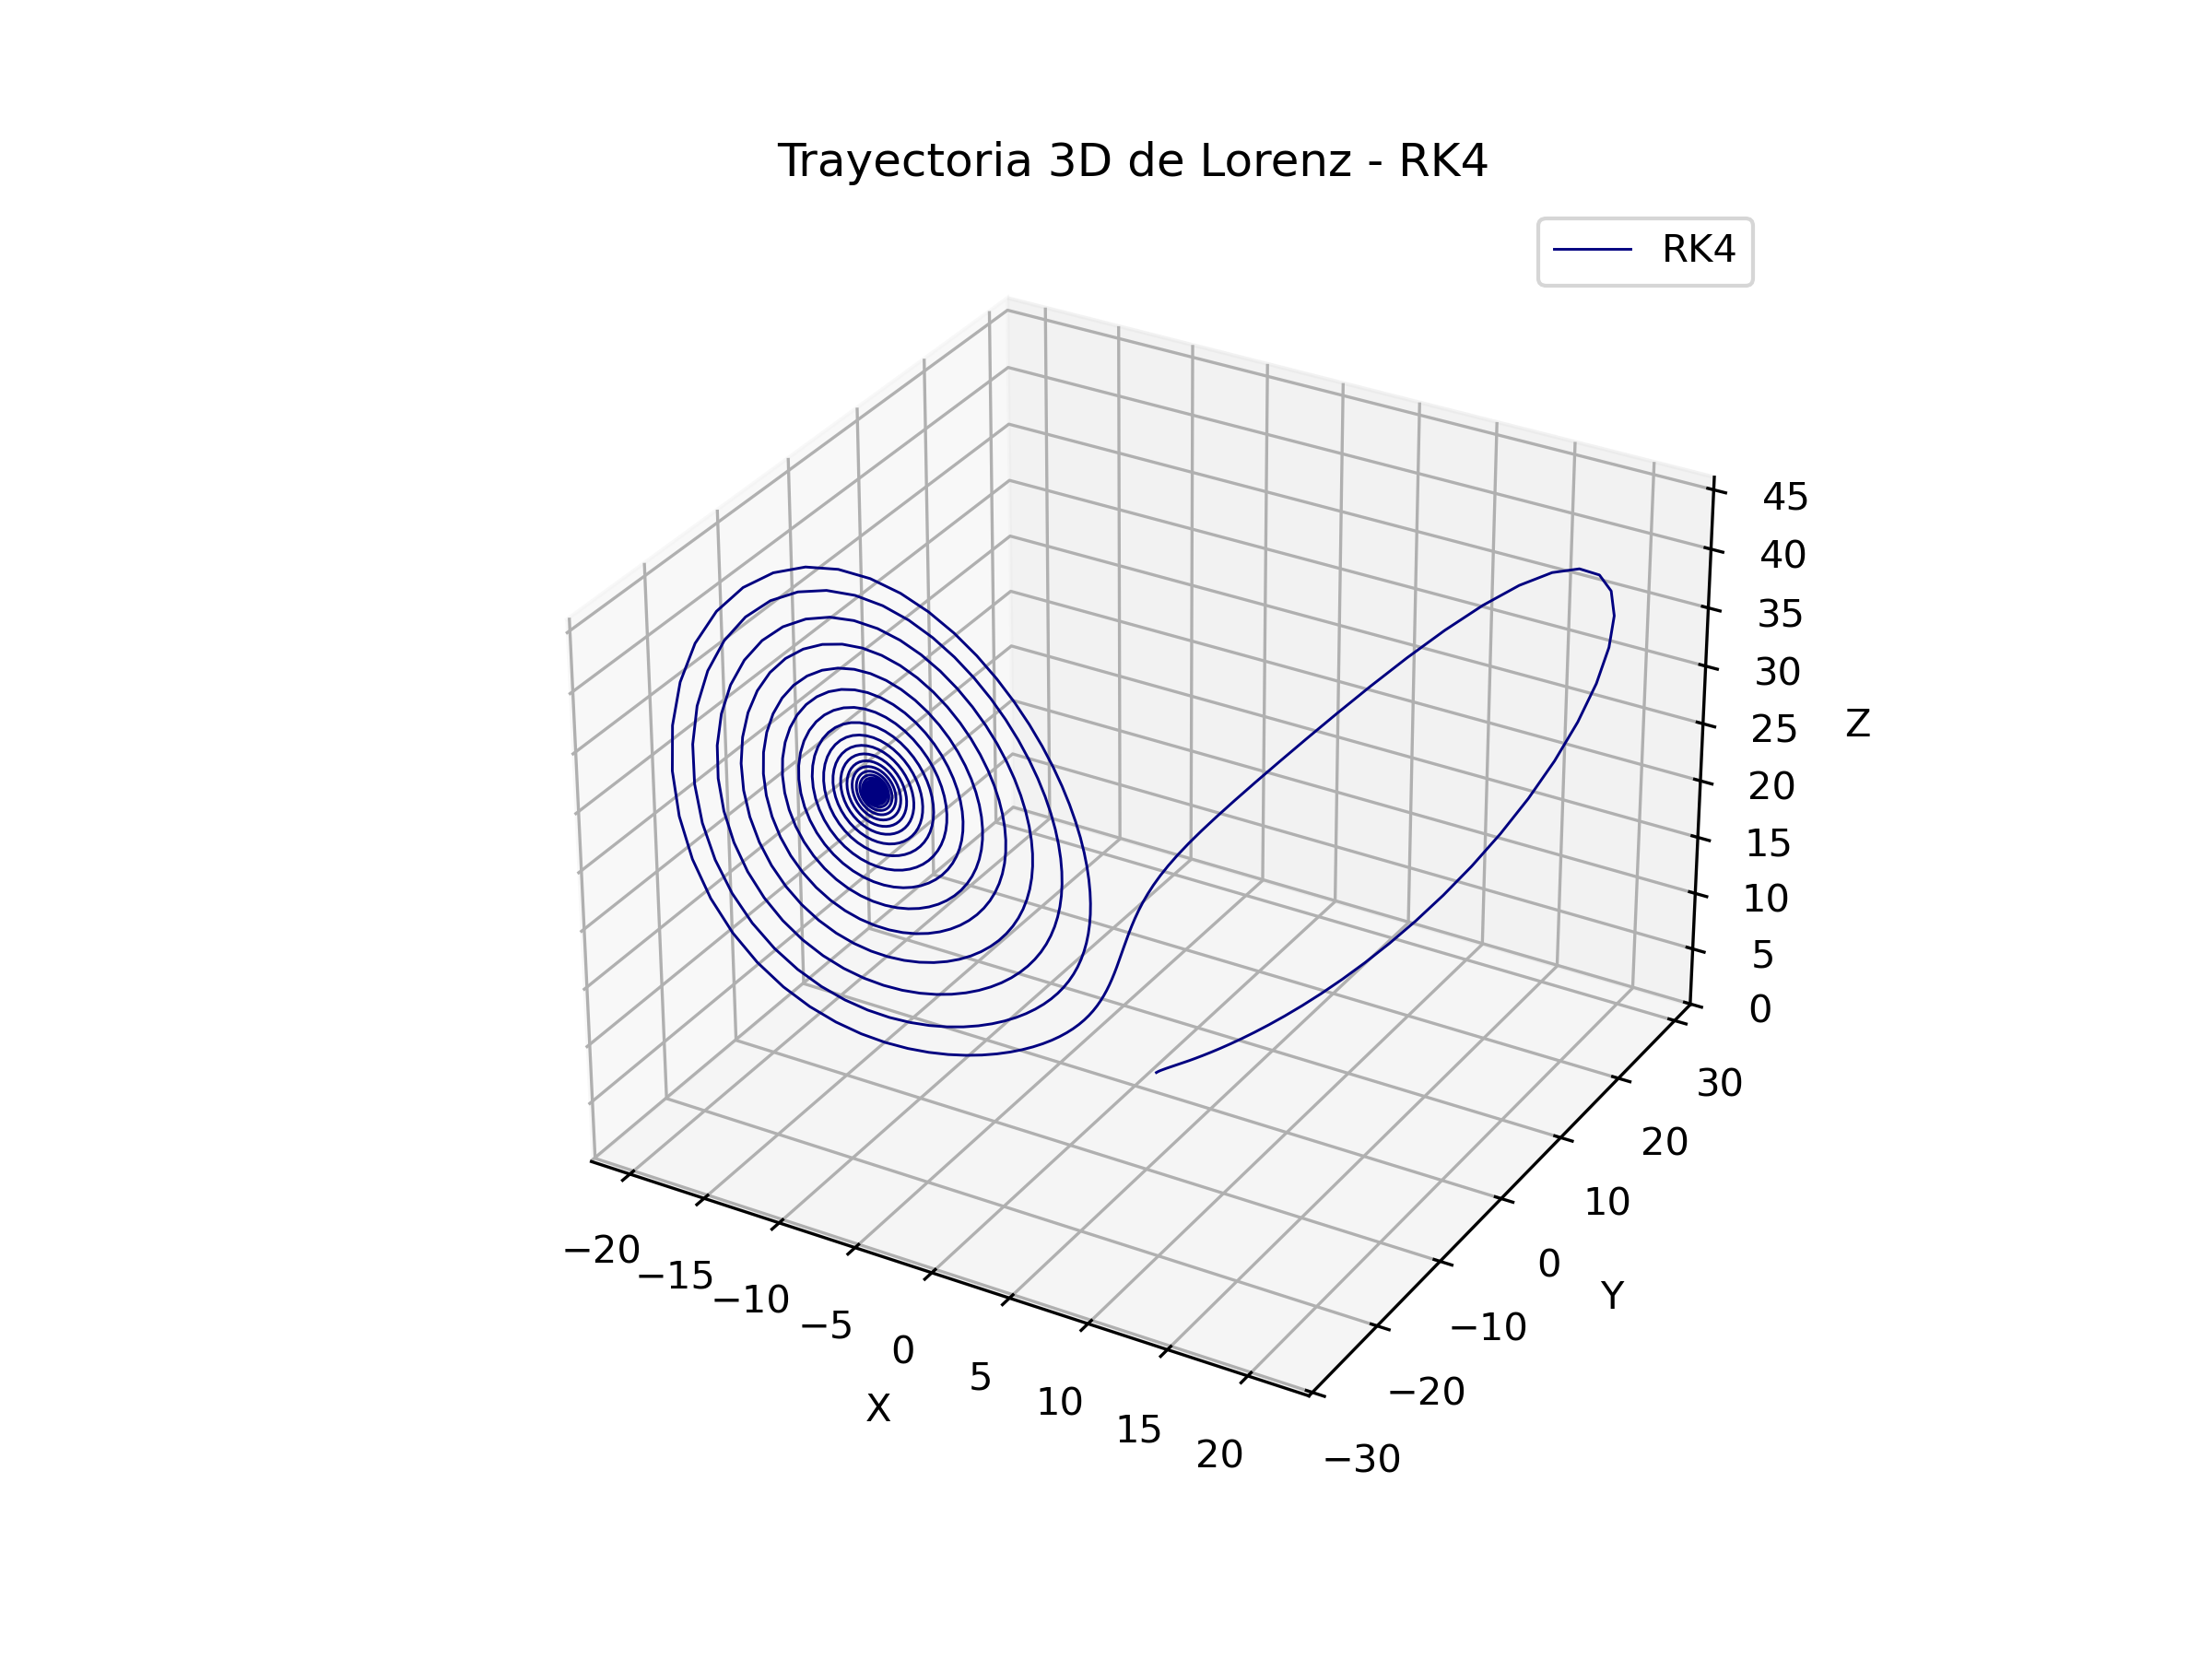
\includegraphics[scale=0.8]{trayectoria_3d_rk4.png}
	\caption{Resultado de la solución de ecuaciones diferenciales (trayectoria) mediante el método RK4}
	\label{fig:RK4}
\end{figure}

\section*{Conclusiones}

Podemos encontrar algunas conclusiones interesantes, las cuales serán enumeradas a continuación: \\

\begin{enumerate}

\item Superioridad de los métodos de alto orden, donde podemos observar que los métodos lineales como el de Euler, pueden generar un error de magnitud considerablemente mayor a diferencia de los métodos de la familia de Runge-Kutta, donde al aumentar el orden, podemos observar que existe una mayor optimización de los resultados y una mayor cercanía de la solución real del método con el tipo de movimiento esperado para una gráfica de este tipo.

\item Tenemos que el sistema de Lorenz tiene naturaleza caótica y que una perturbación puede desencadenar una divergencia exponencial en las trayectorias.

\item Un buen desarrollo de combinación de métodos en Python y C++, gracias a la librería Pybind11, donde podemos ejecutar los trabajos más "pesados" desde un programa en un lenguaje externo como C++ y desarrollar trabajos de graficación con base a lo calculado en dicho método para simplificar el trabajo de Python, al reducir el trabajo matemático que puede en algunas ocasiones saturar el intérprete de este lenguaje de programación.

\end{enumerate}
\end{document}